\section{Halvledardioden}
\textbf{HAREC a.\ref{HAREC.a.2.5}\label{myHAREC.a.2.5}}
\index{halvledardiod}
\index{diod}

\subsection{Allmänt}
I en strömkrets kan av olika anledningar ström tillåtas att flyta i en riktning
men kanske inte i den motsatta. En anordning med en sådan funktion kallas för
diod.

Först bestod en diod av två elektroder i vakuum (se avsnitt
\ref{vakuumdioden}). Därav namnet vakuumdiod.
Numera består en diod oftast av någon halvledare. Därav namnet halvledardiod.

\begin{figure}
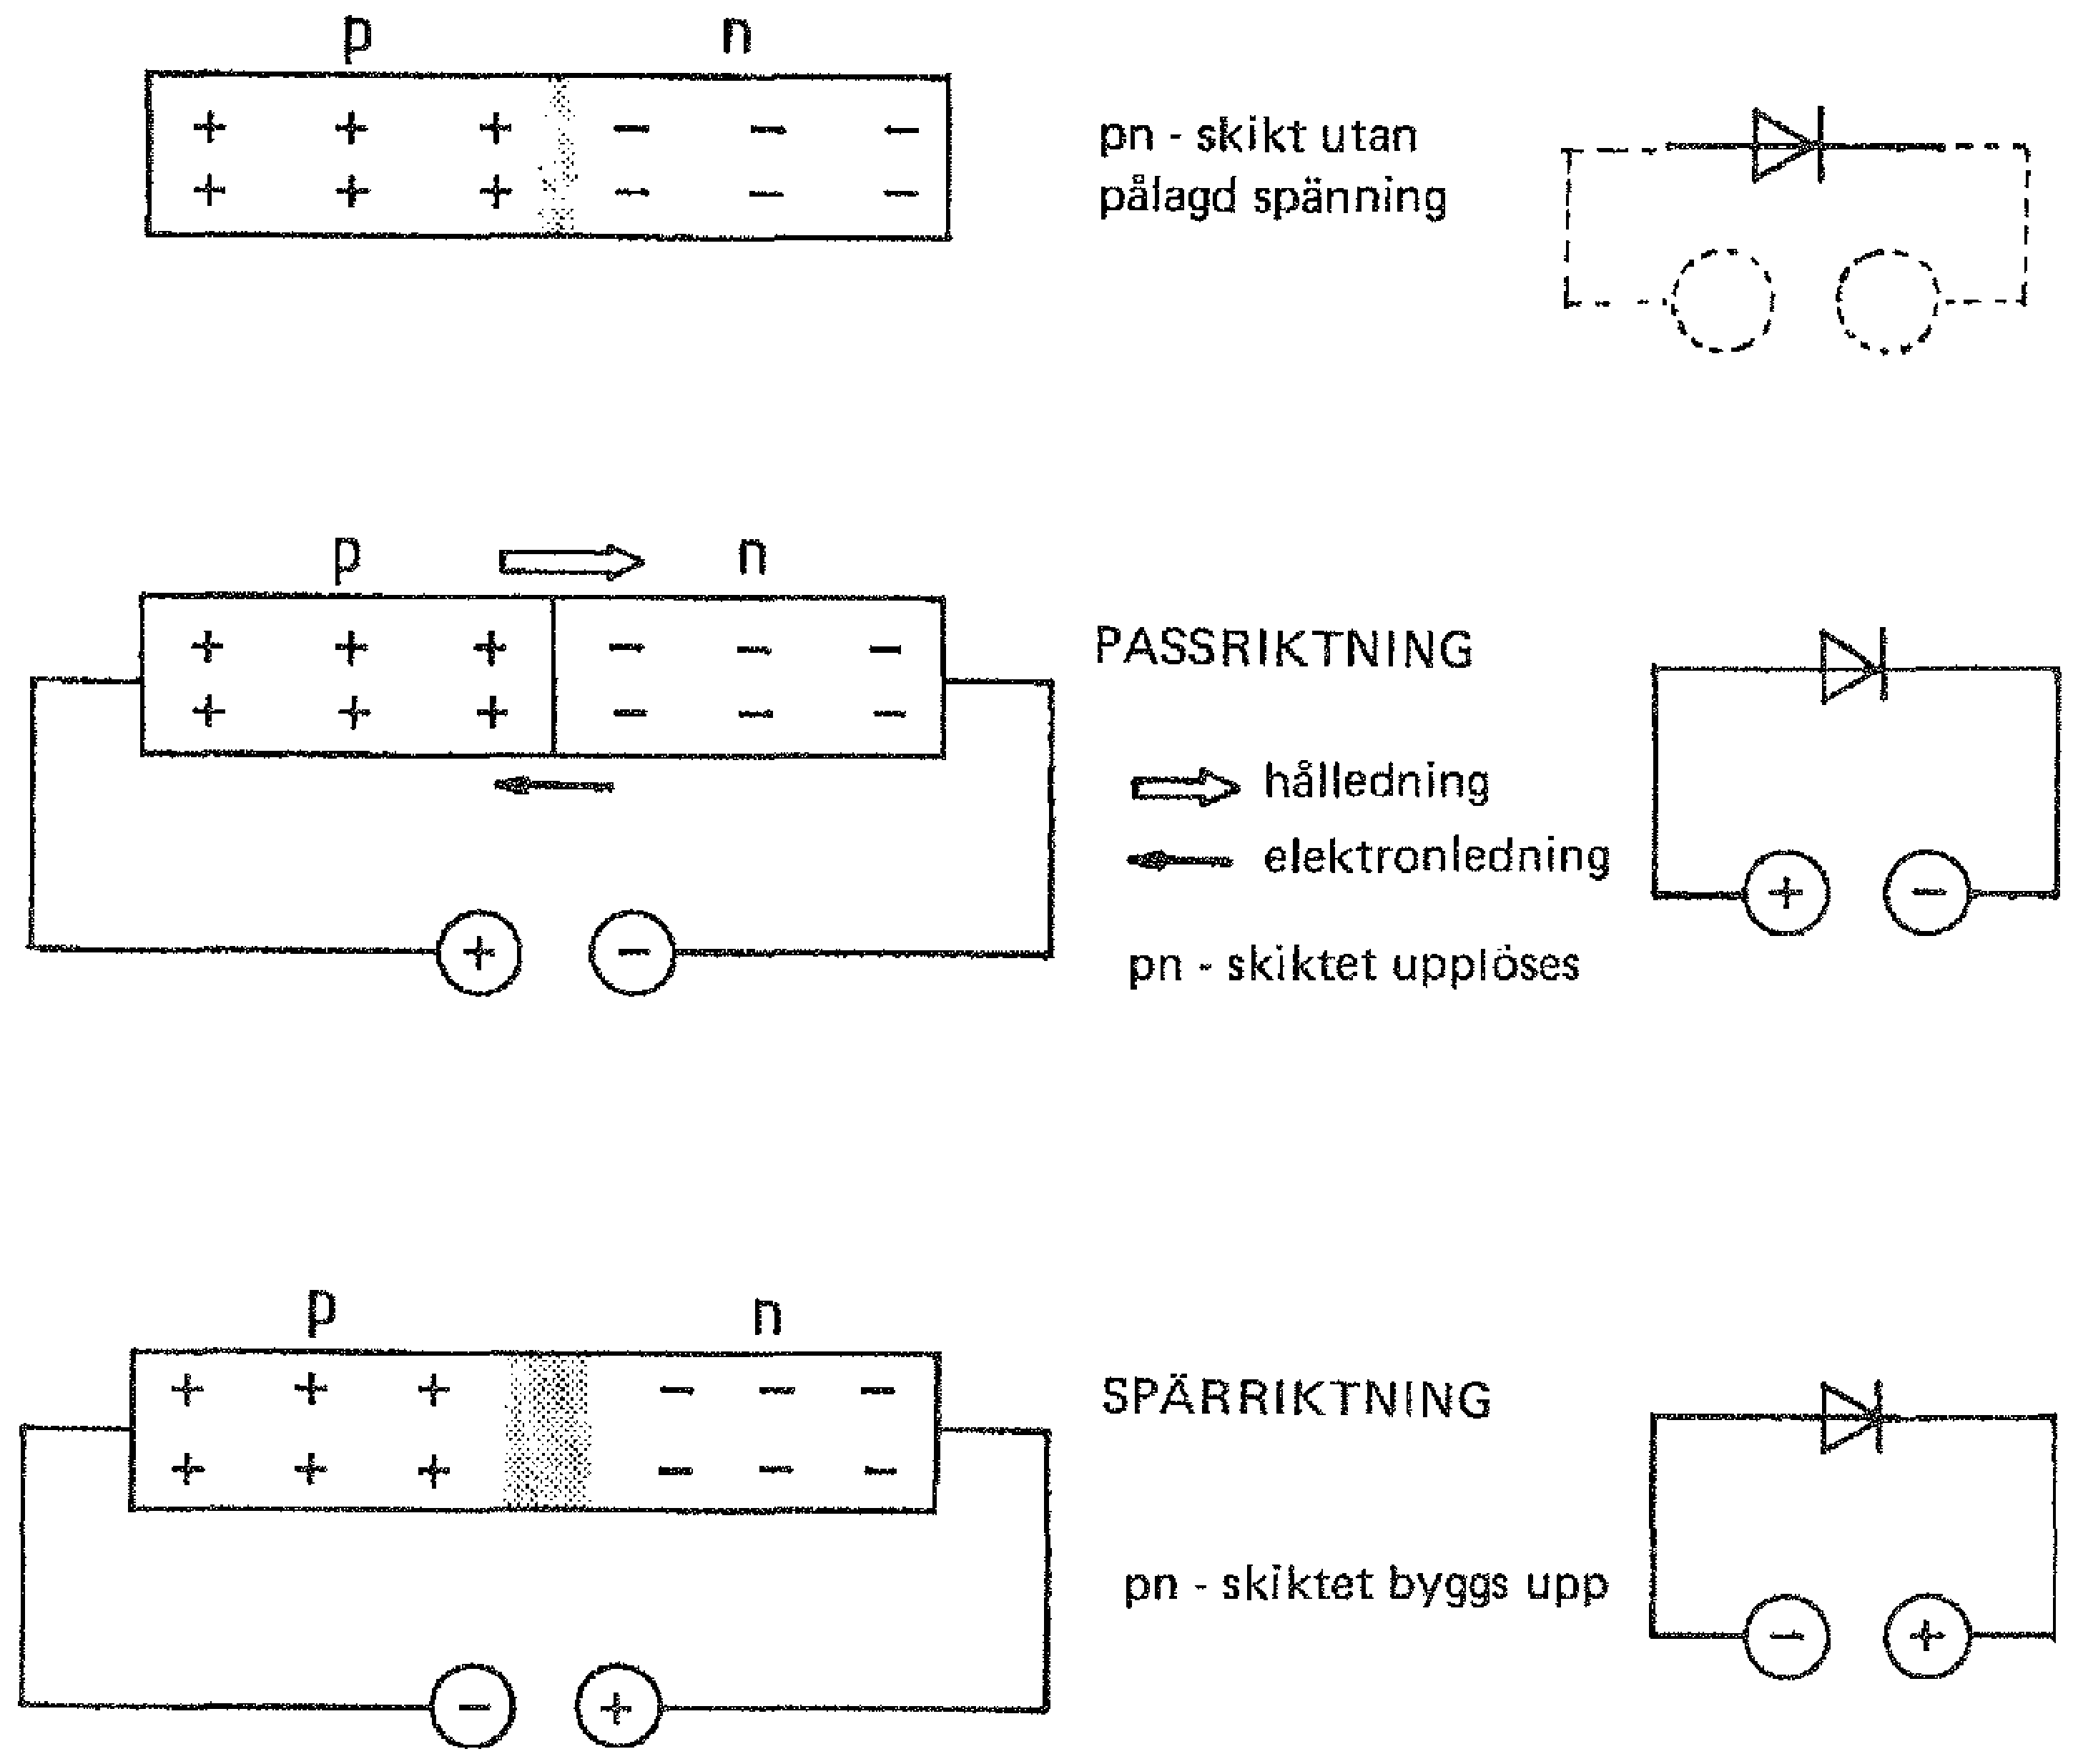
\includegraphics[width=\textwidth]{images/cropped_pdfs/bild_2_2-12.pdf}
\caption{Spärrskiktet i en halvledardiod}
\label{fig:BildII2-12}
\end{figure}

Bild \ref{fig:BildII2-12} överst illustrerar en halvledardiod består av ett
P-ledande och ett N-ledande materialskikt som fogats samman.

Mellan de båda skikten utbildas ett tunt gränsskikt, som inte innehåller
laddningsbärare. Detta skikt kan vara ledande eller icke ledande -- ett
spärrskikt -- beroende på polariseringen.

\subsection{Halvledardiodens karaktär}
\textbf{HAREC a.\ref{HAREC.a.2.5.1.2}\label{myHAREC.a.2.5.1.2}}

\subsubsection{Diod i framriktningen}
\index{framriktning}
\index{framström}
\index{framspänningsfallet}

Förbinder man den positiva polen på en spänningskälla med P-skiktet i en diod
och den negativa polen med N-skiktet så är dioden polariserad i
\emph{framriktningen}, detta illustreras i bild \ref{fig:BildII2-12} mitten.
Spärrskiktet upplöses då och ström flyter genom dioden, dvs. \emph{framström}
(eng. \emph{forward current}).
Elektronerna flyter till den positiva polen och hålen till den negativa polen.
Över anslutningarna ligger en spänning, \emph{framspänningsfallet}
(eng. \emph{forward voltage}), som varierar med strömmen och temperaturen.
Spänningsfallet och strömmen ger på normalt sett diodens \emph{förlusteffekt}.

\subsubsection{Diod i backriktningen}
\index{spärriktningen}
\index{backriktningen}
\index{zenereffekt}

\emph{Backspänning, backström, läckström, spärriktning}

Förbinder man i stället den negativa polen på en spänningskälla med P-skiktet i
en diod och den positiva polen med N-skiktet så är dioden polariserad i
\emph{spärriktningen} eller \emph{backriktningen}, så som illustreras i
bild \ref{fig:BildII2-12} underst.
Spärrskiktet blir då ännu kraftigare.

Endast en obetydlig ström \(I_{SP}\) flyter genom dioden i den s.k.
spärriktningen även vid ökande spänning \(U_{SP}\).
Men över en viss spänning ökar strömmen snabbt -- den s.k. zenereffekten
uppstår.
Dioden kan då lätt förstöras av en alltför hög ström.

\subsubsection{Diodens ström-spänningsförhållande}

\begin{figure}
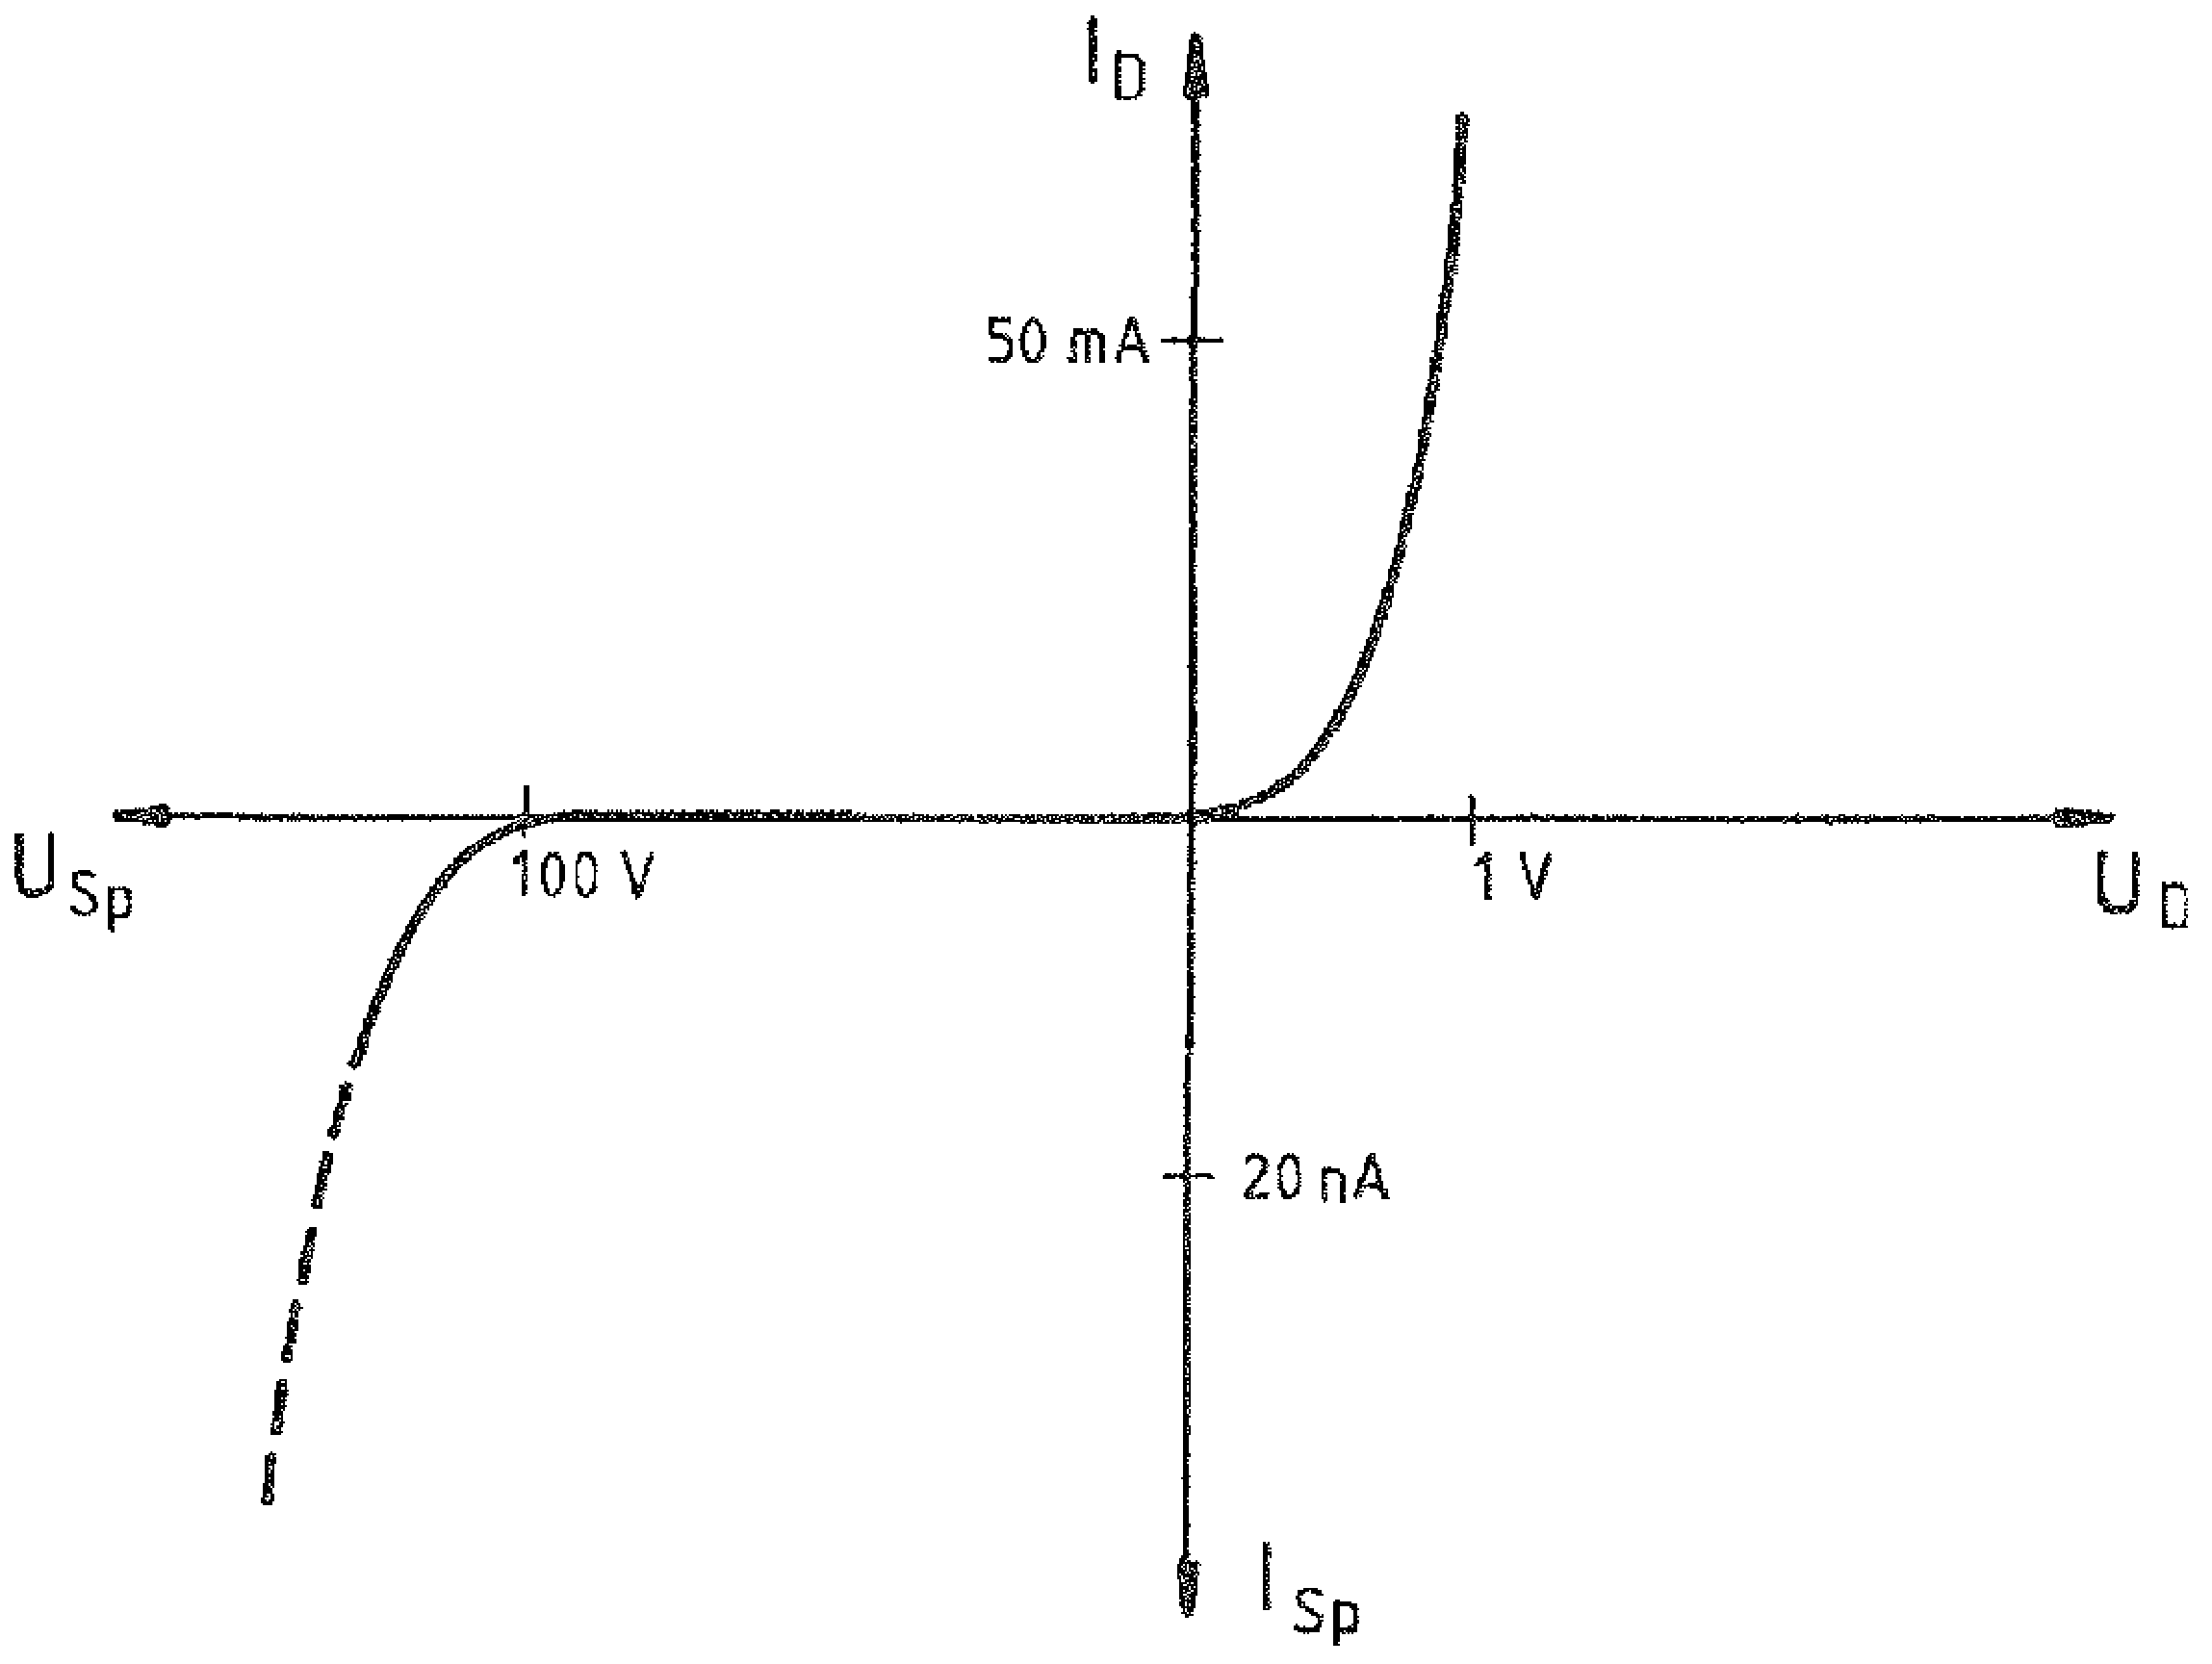
\includegraphics[width=\textwidth]{images/cropped_pdfs/bild_2_2-13.pdf}
\caption{Halvledardiodens karaktäristik}
\label{fig:BildII2-13}
\end{figure}

Bild \ref{fig:BildII2-13} visar en diods ström-spänningsförhållande.

Strömmen \(I_D\) börjar att flyta när spänningen \(U_D\) har nått ett
tröskelvärde (vid kiseldioder 0,6~V).
När spänningen ökar ytterligare däröver, så ökar även strömmen.

Produkten av spänningsfallet över dioden och strömmen genom den kallas
förlusteffekt. Denna värmer upp dioden. Vid för hög temperatur förstörs
kristallstrukturen. En kiselkristall kan klara upp till 200~\degree C medan en
germaniumkristall bara klarar 75~\degree C.

\subsection{Diodtillämpningar}
\textbf{HAREC a.\ref{HAREC.a.2.5.1.1}\label{myHAREC.a.2.5.1.1}}

Bild \ref{fig:BildII2-14} illustrerar flera olika schema-symboler för
dioder.

\begin{wrapfigure}[13]{R}{0.5\textwidth}
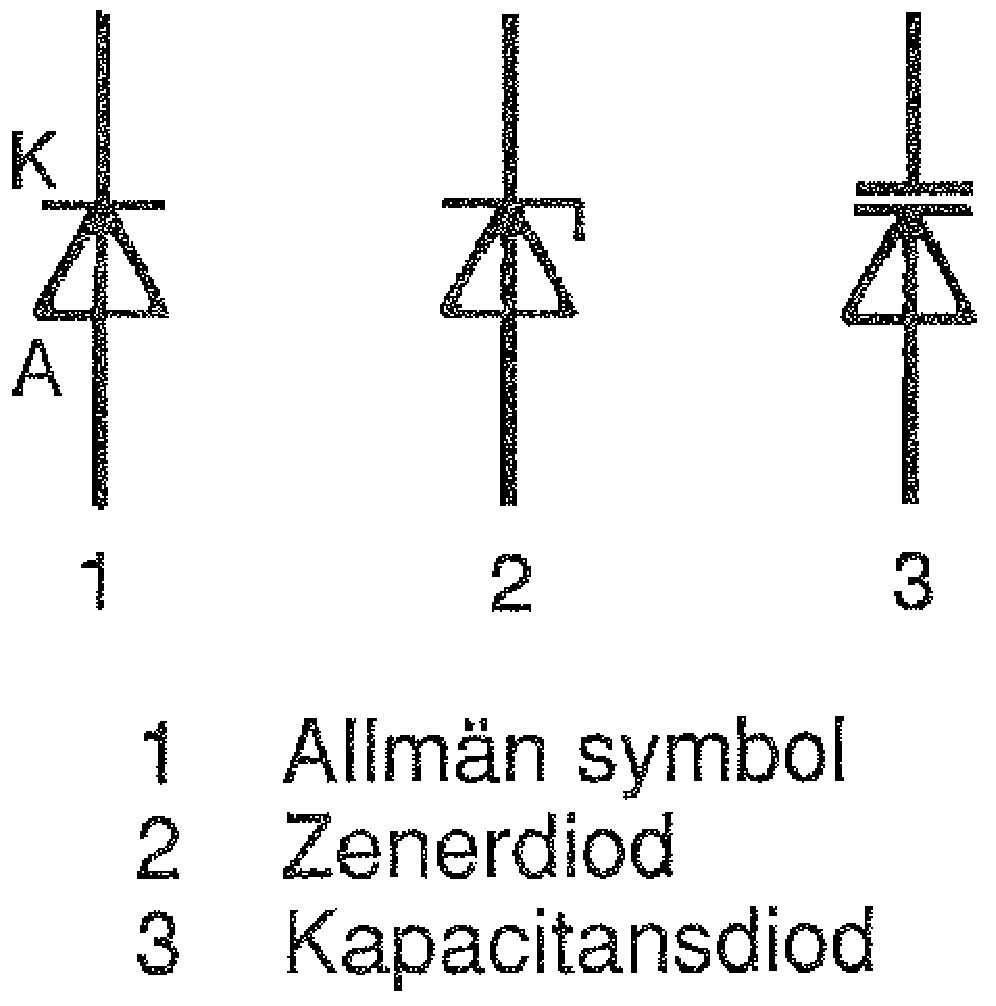
\includegraphics[width=0.5\textwidth]{images/cropped_pdfs/bild_2_2-14.pdf}
\caption{Schemasymboler för dioder}
\label{fig:BildII2-14}
\end{wrapfigure}

Likriktning är det vanligaste tillämpningen (se kapitel \ref{kraftaggregat}).
Halvledardioder görs även för en rad andra ändamål och finns i en mängd
utföranden, så som

\subsubsection{Dioder för spänningsstabilisering (zenerdiod).}
\index{zenerdiod}
\index{diod!zener}

  Inom ett visst område är spänningsfallet över en zenerdiod i en strömkrets
  i det närmaste konstant medan strömmen varierar. Denna egenskap kallas
  zenereffekt och används för konstanthållning av spänning.

  Det finns zenerdioder många olika spänningar och effekter.

\subsubsection{Dioder som variabel kondensator, s.k. kapacitansdiod (VariCap)}
\label{varicap}
\index{varicap}
\index{diod!varicap}

  När en diod är polariserad i spärriktningen så bildas det ett spärrskikt.
  Olika polariseringsspänning alstrar olika tjocka spärrskikt En spärrad diod
  har på så sätt egenskaper som liknar dem i en variabel kondensator. Det finns
  därför dioder där reglerbarheten av kapacitansen är speciellt utvecklad.

\subsubsection{Lysdioder (LED)}
\index{lysdioder}
\index{diod!lysdiod}
\index{LED}
\index{diod!LED}
\index{laserdiod}
\index{diod!laserdiod}

\emph{Lysdiod} (eng. \emph{Light Emitting Diode (LED)}) är en diod anpassad för
att leverera ljus, ofta synligt.
Lysdioder finns tillgängliga med infrarött, rött, orange, gult, grönt,
blått och vitt ljus.
En variant av lysdiod är laserdioder, som bland annat används för överföring
över optisk fiber.

Energi frigörs i spärrzonen i en diod som är polariserad i passriktningen.
Det sker genom rekombination av par av laddningsbärare, varvid det normalt avgår
energi i form av värme.
Vid en viss inblandning av främmande atomer avgår istället ljus.

Spänningfallet över en lysdiod är ungefär dubbelt så stort som över en
kiseldiod, dvs. ungefär 1,5~volt.
Det normala spänningsfallet bör alltid kontrolleras för korrekt dimensionering
av kretsen.
Strömmen är i proportion med önskad ljusstyrka och mellan 10 och 50~mA.
En lysdiod bör ha ett strömbegränsande motstånd i serie för att strömmen
inte ska bli för stor och lysdioden åldras i förtid eller rent av går
sönder.

Moderna powerled kräver en konstantströmsmatning och kan ha betydligt
högre spänning.
Dessa har blivit tillgängliga till lågt pris och populära för experiment.

\subsection{Vakuumdioden jämfört halvledardioden}

\begin{figure}
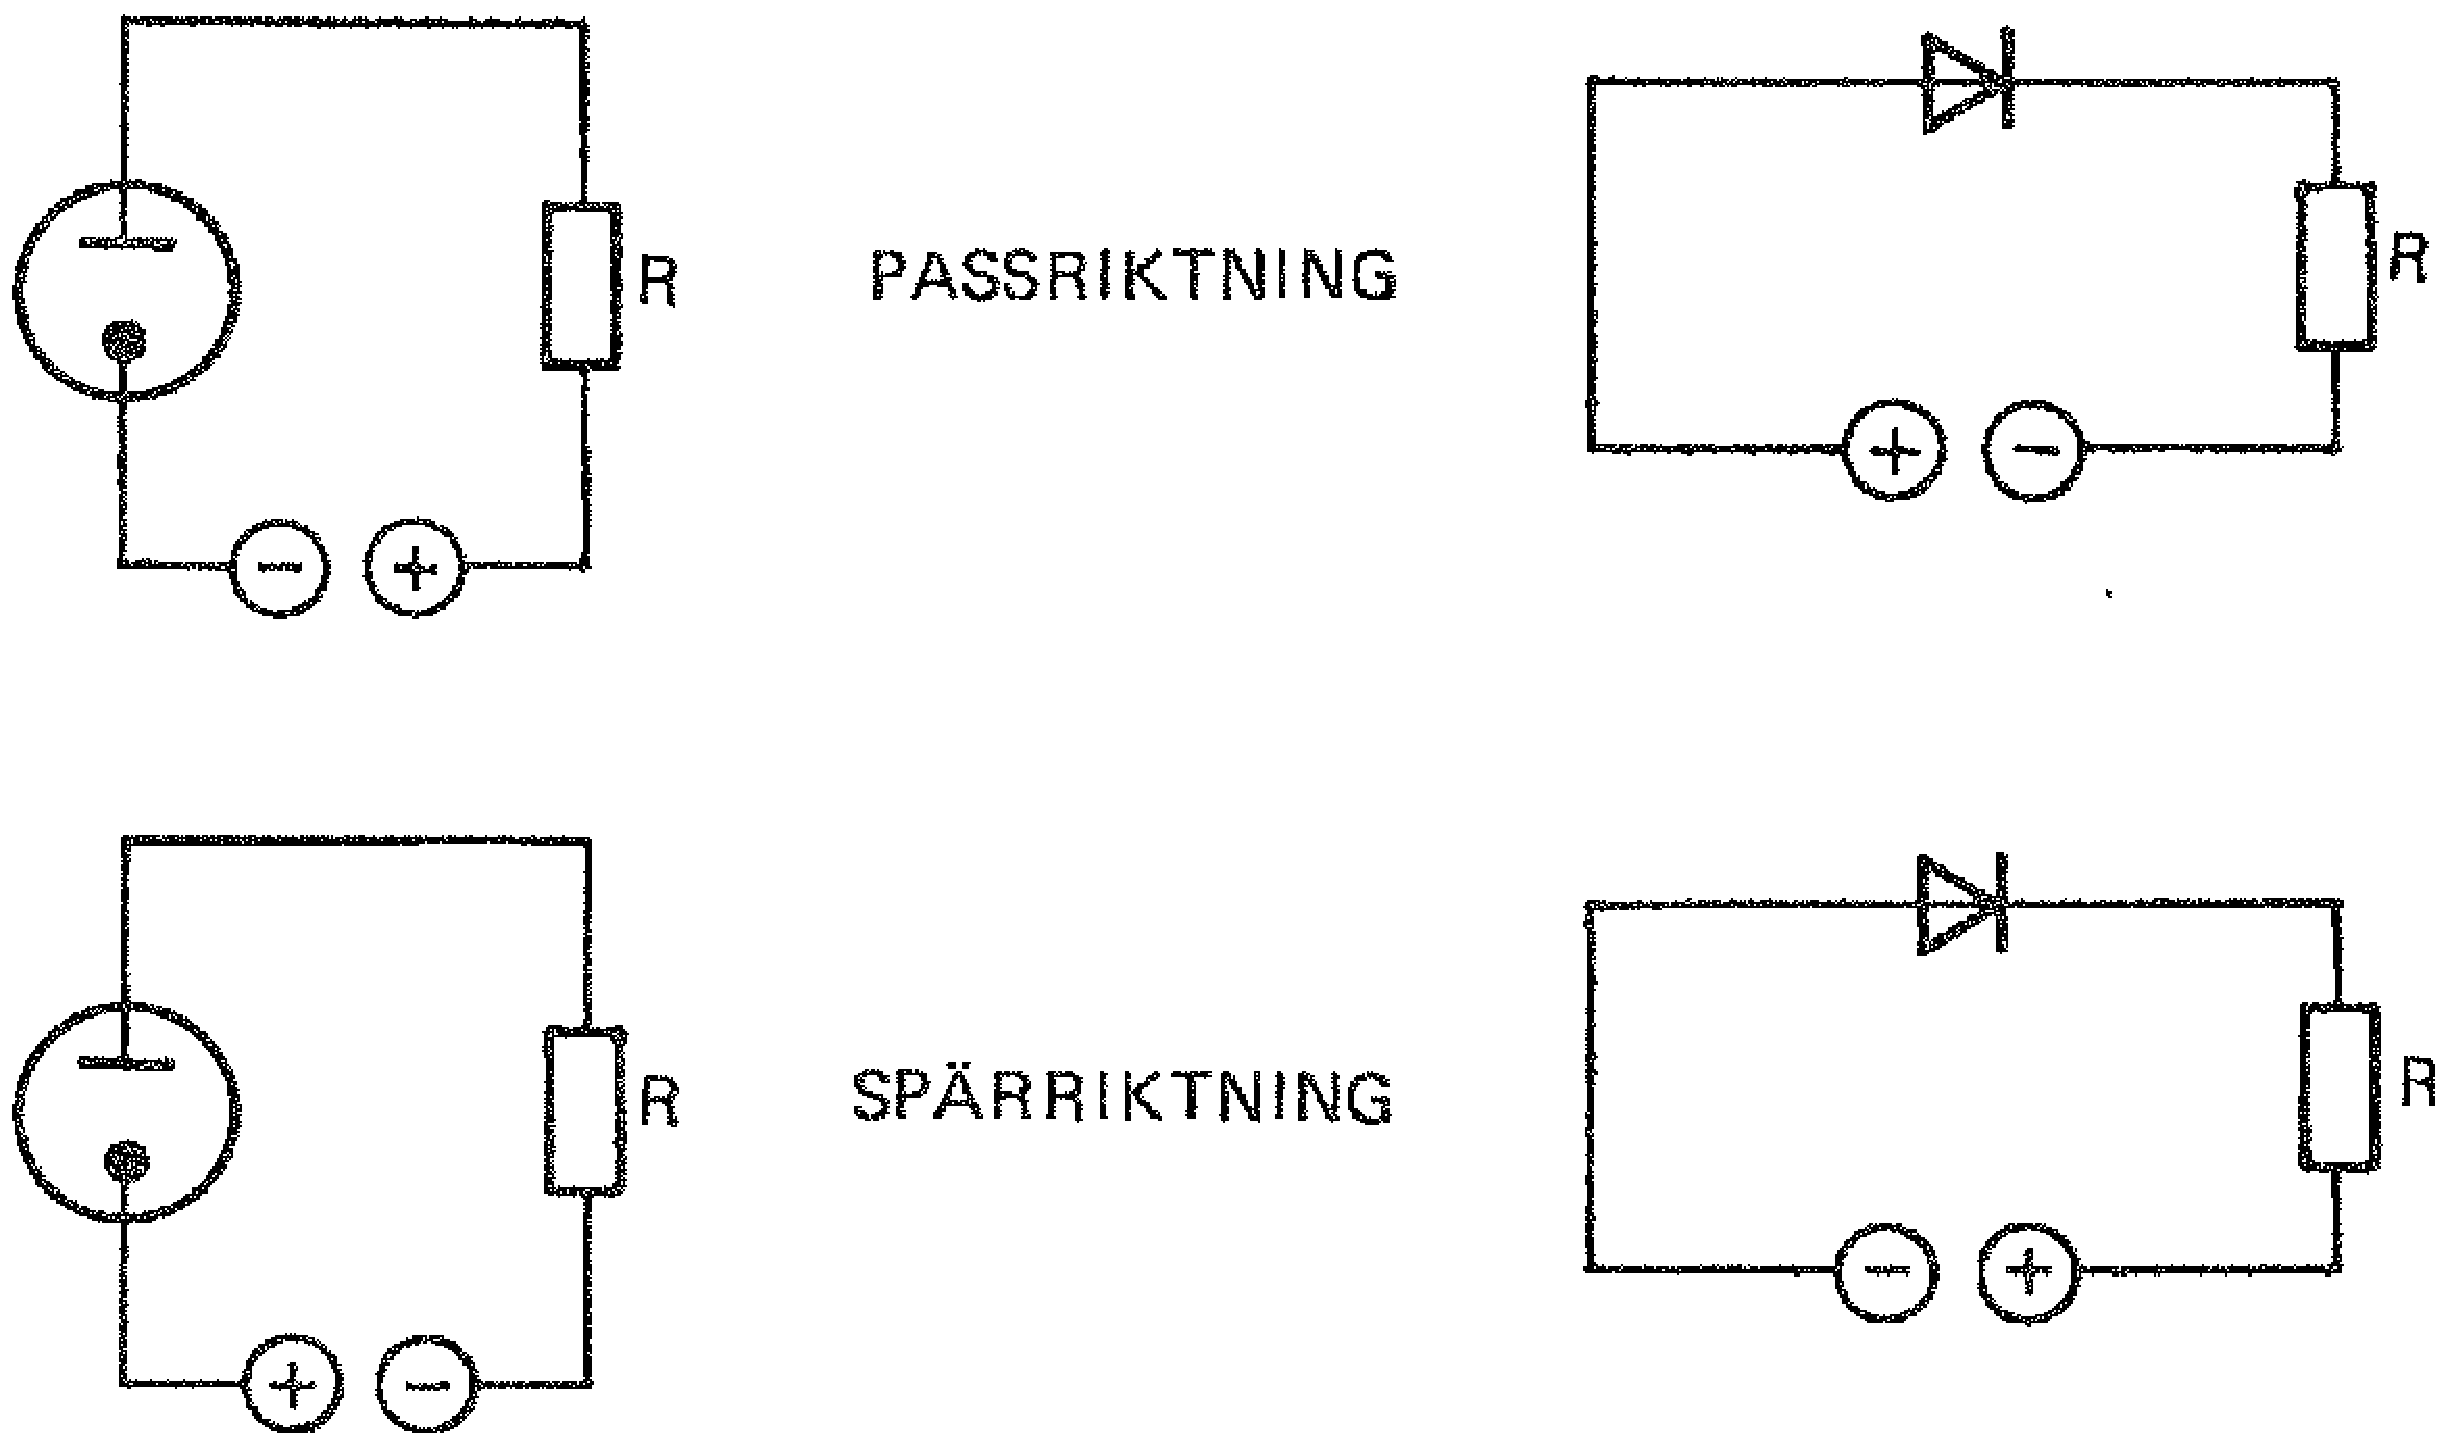
\includegraphics[width=\textwidth]{images/cropped_pdfs/bild_2_2-15.pdf}
\caption{Dioders polarisering i kretsen}
\label{fig:BildII2-15}
\end{figure}

Bild \ref{fig:BildII2-15} visar principen för hur de båda diodtyperna ingår i
en strömkrets.
Den stora skillnaden är att arbetsspänningen för en vakuumdiod är mångfalt
högre än den för en halvledardiod samt att vakuumdiodens ena elektrod (katoden)
behöver hettas upp för att avge elektroner.
